\documentclass{article}


\topmargin=-0.45in      %
\evensidemargin=0in     %
\oddsidemargin=0in      %
\textwidth=6.5in        %
\textheight=9.0in       %
\headsep=0.25in         %


\usepackage{graphicx,float,wrapfig}
\usepackage{moreverb} % monospace
\usepackage{fancyhdr} % fancy header 
\usepackage{lastpage} % last page 
\usepackage{setspace} % line spacing
\usepackage{amsmath,amsfonts,amsthm,amssymb}  % math fonts 
\usepackage{tabularx} % advanced tables
\usepackage[unicode=true] {hyperref}
%%% default Rstudio packages %%%

\usepackage[sort]{natbib}  %% will alpha/numeric in order inline
	\setcitestyle{aysep={}} %% no year, comma just year
	
	
\newcommand{\hmwkCourse}{ \textbf{STATS 419 Survey of Multivariate Analysis} }
\newcommand{\hmwkCourseShort}{STATS419}
\newcommand{\hmwkTitle}{Week 03 Assignment}
\newcommand{\hmwkAuthor}{joshua Bennett}
\newcommand{\hmwkEmail}{joshua.r.bennett@wsu.edu}
\newcommand{\hmwkWSU}{[11373111]}
\newcommand{\hmwkInstructor}{Instructor: Monte J. Shaffer}
\newcommand{\hmwkDate}{16 September 2020}


\pagestyle{fancy}   
\lhead{\hmwkCourseShort}
\chead{\hmwkTitle}
\rhead{\hmwkAuthor}
\lfoot{}
\cfoot{Page\ \thepage\ of\ \protect\pageref{LastPage}}
\rfoot{}



\title{\hmwkCourse \\ \hmwkTitle}
\author{\hmwkAuthor \\ (\hmwkEmail) \\ \hmwkWSU \\[0.5in] \hmwkInstructor }
\date{\hmwkDate}


\usepackage{titling}
\pretitle{\begin{flushright}\LARGE}
\posttitle{\par\end{flushright}\vskip 0.5em}
\preauthor{\begin{flushright}\large \lineskip 0.5em}
\postauthor{\par\end{flushright}}
\predate{\begin{flushright}\large}
\postdate{\par\end{flushright}}


%\tracingall



\begin{document}

\maketitle

%\begin{abstract}
%The abstract text goes here.
%\end{abstract}

\section{Introduction}
Here is the text\footnote{Here is a footnote} of your introduction.

Malcolm Gladwell talks about outliers \citep{Gladwell:2008}.

\begin{equation}
    \label{simple_equation}
    \alpha = \sqrt{ \beta }
\end{equation}

\subsection{Subsection Heading Here}
Write your subsection text here.

\begin{figure}
    \centering
    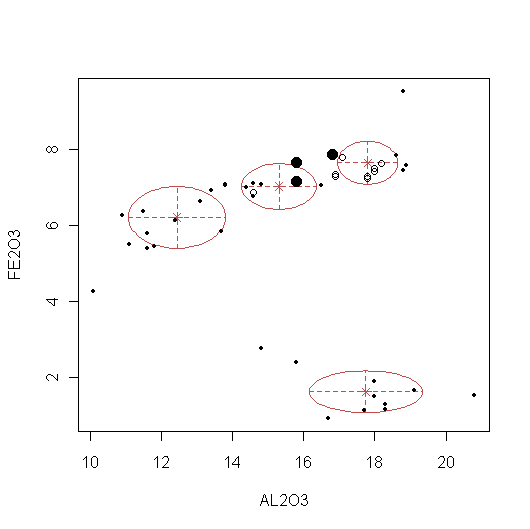
\includegraphics[width=3.0in] {C:/Users/Galac/Desktop/git419/Stats419_FALL2020/LateX/full-example/graphics/myfigure}
   
    \caption{Simulation Results}
    \label{simulationfigure}
\end{figure}


\begin{figure}
    \centering
    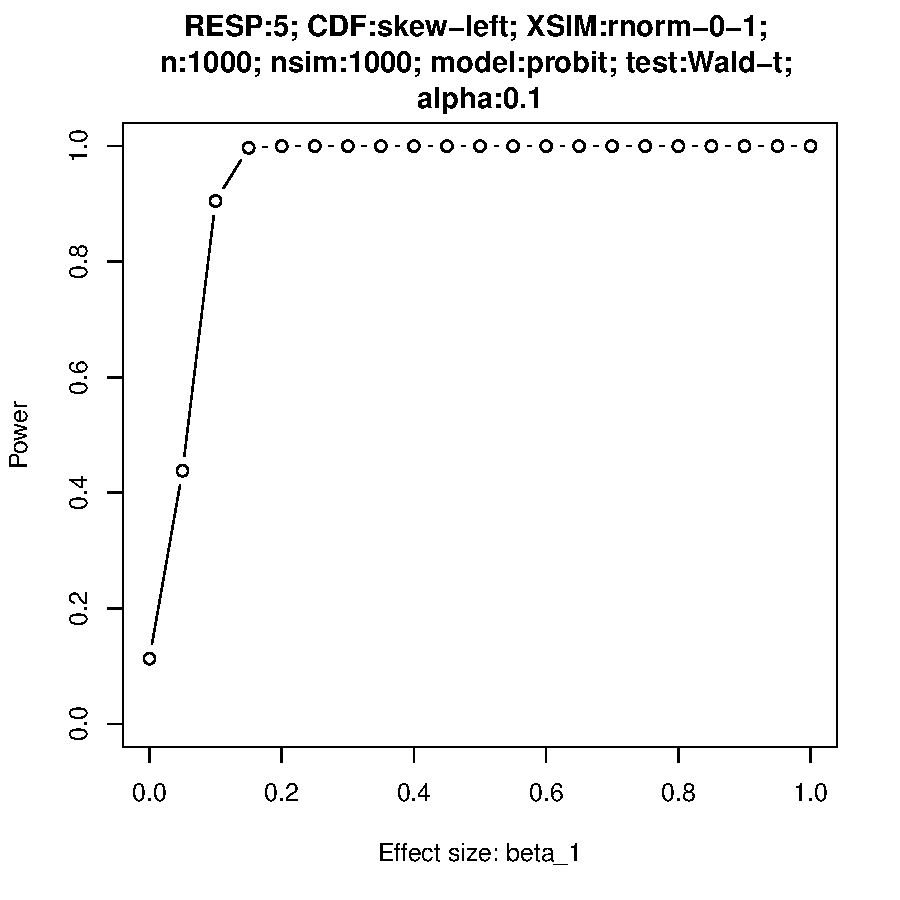
\includegraphics[width=3.0in] {C:/Users/Galac/Desktop/git419/Stats419_FALL2020/LateX/full-example/graphics/pdffigure}
    \caption{Simulation Results PDF}
    \label{simulationfigurepdf}
\end{figure}

\section{Conclusion}
Write your conclusion here.

\begin{Shaded}
\begin{Highlighting}[]
\CommentTok{# plot function here ...}
\KeywordTok{plot}\NormalTok{(iris);}
\end{Highlighting}
\end{Shaded}

\includegraphics{assignment_files/figure-latex/mychunk-iris-demo-1.pdf}

\begin{Shaded}
\begin{Highlighting}[]
\KeywordTok{plot}\NormalTok{(iris[,}\OperatorTok{-}\DecValTok{5}\NormalTok{]);}
\end{Highlighting}
\end{Shaded}

\includegraphics{assignment_files/figure-latex/mychunk-iris-demo-2.pdf}

\begin{Shaded}
\begin{Highlighting}[]
\KeywordTok{plot}\NormalTok{(iris[,}\OperatorTok{-}\DecValTok{5}\NormalTok{],}\DataTypeTok{col=}\NormalTok{iris[,}\DecValTok{5}\NormalTok{]);}
\end{Highlighting}
\end{Shaded}

\includegraphics{assignment_files/figure-latex/mychunk-iris-demo-3.pdf}

\begin{Shaded}
\begin{Highlighting}[]
\KeywordTok{levels}\NormalTok{(iris[,}\DecValTok{5}\NormalTok{]);}
\end{Highlighting}
\end{Shaded}

\begin{verbatim}
## [1] "setosa"     "versicolor" "virginica"
\end{verbatim}

\begin{Shaded}
\begin{Highlighting}[]
\NormalTok{myColors =}\StringTok{ }\KeywordTok{c}\NormalTok{(}\StringTok{"red"}\NormalTok{,}\StringTok{"green"}\NormalTok{,}\StringTok{"blue"}\NormalTok{);}
\KeywordTok{plot}\NormalTok{(iris[,}\OperatorTok{-}\DecValTok{5}\NormalTok{],}\DataTypeTok{col=}\NormalTok{myColors);}
\end{Highlighting}
\end{Shaded}

\includegraphics{assignment_files/figure-latex/mychunk-iris-demo-4.pdf}

\begin{Shaded}
\begin{Highlighting}[]
\NormalTok{species =}\StringTok{ }\KeywordTok{as.numeric}\NormalTok{(iris[,}\DecValTok{5}\NormalTok{]);}

\KeywordTok{as.numeric}\NormalTok{(iris[,}\DecValTok{5}\NormalTok{]);  }\CommentTok{# map to myColors ...}
\end{Highlighting}
\end{Shaded}

\begin{verbatim}
##   [1] 1 1 1 1 1 1 1 1 1 1 1 1 1 1 1 1 1 1 1 1 1 1 1 1 1 1 1 1 1 1 1 1 1 1 1 1 1
##  [38] 1 1 1 1 1 1 1 1 1 1 1 1 1 2 2 2 2 2 2 2 2 2 2 2 2 2 2 2 2 2 2 2 2 2 2 2 2
##  [75] 2 2 2 2 2 2 2 2 2 2 2 2 2 2 2 2 2 2 2 2 2 2 2 2 2 2 3 3 3 3 3 3 3 3 3 3 3
## [112] 3 3 3 3 3 3 3 3 3 3 3 3 3 3 3 3 3 3 3 3 3 3 3 3 3 3 3 3 3 3 3 3 3 3 3 3 3
## [149] 3 3
\end{verbatim}

\begin{Shaded}
\begin{Highlighting}[]
\NormalTok{species =}\StringTok{ }\KeywordTok{as.numeric}\NormalTok{(iris[,}\DecValTok{5}\NormalTok{]);}
\NormalTok{myColors[species]}
\end{Highlighting}
\end{Shaded}

\begin{verbatim}
##   [1] "red"   "red"   "red"   "red"   "red"   "red"   "red"   "red"   "red"  
##  [10] "red"   "red"   "red"   "red"   "red"   "red"   "red"   "red"   "red"  
##  [19] "red"   "red"   "red"   "red"   "red"   "red"   "red"   "red"   "red"  
##  [28] "red"   "red"   "red"   "red"   "red"   "red"   "red"   "red"   "red"  
##  [37] "red"   "red"   "red"   "red"   "red"   "red"   "red"   "red"   "red"  
##  [46] "red"   "red"   "red"   "red"   "red"   "green" "green" "green" "green"
##  [55] "green" "green" "green" "green" "green" "green" "green" "green" "green"
##  [64] "green" "green" "green" "green" "green" "green" "green" "green" "green"
##  [73] "green" "green" "green" "green" "green" "green" "green" "green" "green"
##  [82] "green" "green" "green" "green" "green" "green" "green" "green" "green"
##  [91] "green" "green" "green" "green" "green" "green" "green" "green" "green"
## [100] "green" "blue"  "blue"  "blue"  "blue"  "blue"  "blue"  "blue"  "blue" 
## [109] "blue"  "blue"  "blue"  "blue"  "blue"  "blue"  "blue"  "blue"  "blue" 
## [118] "blue"  "blue"  "blue"  "blue"  "blue"  "blue"  "blue"  "blue"  "blue" 
## [127] "blue"  "blue"  "blue"  "blue"  "blue"  "blue"  "blue"  "blue"  "blue" 
## [136] "blue"  "blue"  "blue"  "blue"  "blue"  "blue"  "blue"  "blue"  "blue" 
## [145] "blue"  "blue"  "blue"  "blue"  "blue"  "blue"
\end{verbatim}

\begin{Shaded}
\begin{Highlighting}[]
\KeywordTok{plot}\NormalTok{(iris[,}\OperatorTok{-}\DecValTok{5}\NormalTok{],}\DataTypeTok{col=}\NormalTok{myColors[species]);}
\end{Highlighting}
\end{Shaded}

\includegraphics{assignment_files/figure-latex/mychunk-iris-demo-5.pdf}

\begin{Shaded}
\begin{Highlighting}[]
\KeywordTok{plot}\NormalTok{(iris[,}\OperatorTok{-}\DecValTok{5}\NormalTok{],}\DataTypeTok{col=}\NormalTok{myColors[species], }\DataTypeTok{pch=}\DecValTok{19}\NormalTok{);}
\end{Highlighting}
\end{Shaded}

\includegraphics{assignment_files/figure-latex/mychunk-iris-demo-6.pdf}

\begin{Shaded}
\begin{Highlighting}[]
\NormalTok{myColors =}\StringTok{ }\KeywordTok{c}\NormalTok{(}\StringTok{"red"}\NormalTok{,}\StringTok{"green"}\NormalTok{,}\StringTok{"blue"}\NormalTok{);}
\NormalTok{mySymbols =}\StringTok{ }\KeywordTok{c}\NormalTok{(}\DecValTok{15}\NormalTok{, }\DecValTok{16}\NormalTok{, }\DecValTok{18}\NormalTok{);}
\NormalTok{species =}\StringTok{ }\KeywordTok{as.numeric}\NormalTok{(iris[,}\DecValTok{5}\NormalTok{]);}
\KeywordTok{plot}\NormalTok{(iris[,}\OperatorTok{-}\DecValTok{5}\NormalTok{],}\DataTypeTok{col=}\NormalTok{myColors[species], }\DataTypeTok{pch=}\NormalTok{mySymbols[species]);}
\end{Highlighting}
\end{Shaded}

\includegraphics{assignment_files/figure-latex/mychunk-iris-demo-7.pdf}

\begin{Shaded}
\begin{Highlighting}[]
\CommentTok{#legend("bottomright",unique(species),col=myColors[species],pch=mySymbols[species]);  # why is legend not working?}




\CommentTok{# final answer using plot}
\NormalTok{myColors =}\StringTok{ }\KeywordTok{c}\NormalTok{(}\StringTok{"red"}\NormalTok{,}\StringTok{"green"}\NormalTok{,}\StringTok{"blue"}\NormalTok{);}
\NormalTok{mySymbols =}\StringTok{ }\KeywordTok{c}\NormalTok{(}\DecValTok{19}\NormalTok{, }\DecValTok{19}\NormalTok{, }\DecValTok{19}\NormalTok{);}
\NormalTok{species =}\StringTok{ }\KeywordTok{as.numeric}\NormalTok{(iris[,}\DecValTok{5}\NormalTok{]);}
\KeywordTok{plot}\NormalTok{( iris[,}\OperatorTok{-}\DecValTok{5}\NormalTok{],}
      \DataTypeTok{col=}\NormalTok{myColors[species], }
      \DataTypeTok{pch=}\NormalTok{mySymbols[species],}
      \DataTypeTok{main=}\StringTok{"Iris Data (red=setosa,green=versicolor,blue=virginica)"}
\NormalTok{    );}
\end{Highlighting}
\end{Shaded}

\includegraphics{assignment_files/figure-latex/mychunk-iris-demo-8.pdf}

\begin{Shaded}
\begin{Highlighting}[]
\CommentTok{# we need to add a caption into our final answer of our writeup ...  ALWAYS ...}


\CommentTok{## R Markdown}
\end{Highlighting}
\end{Shaded}

\hypertarget{including-plots}{%
\subsection{Including Plots}\label{including-plots}}

You can also embed plots, for example:

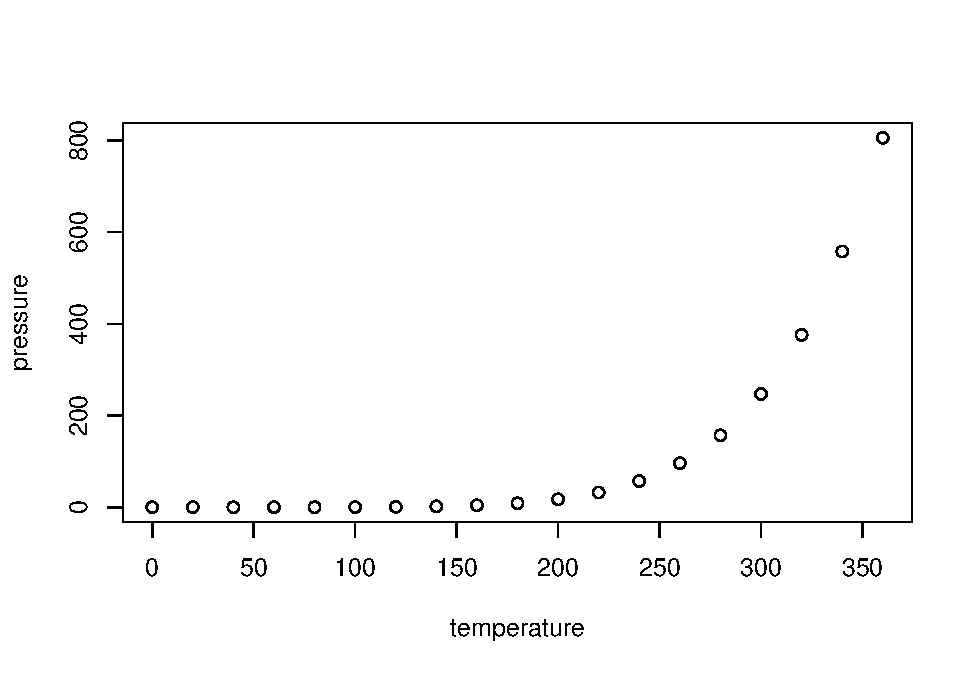
\includegraphics{assignment_files/figure-latex/pressure-1.pdf}

Note that the \texttt{echo\ =\ FALSE} parameter was added to the code
chunk to prevent printing of the R code that generated the plot.


\newpage
\bibliographystyle{biblio/chicagoAMA}
\bibliography{biblio/master} % this is master.bib located in the biblio subfolder ... you could have multiple files here if need be ... one is easier ...


\end{document}